\documentclass[12pt,a4paper]{report}
\usepackage[utf8]{inputenc}
\usepackage[spanish]{babel}
\usepackage{geometry}
\geometry{a4paper, margin=1in}
\usepackage{graphicx}
\usepackage{hyperref}
\usepackage{lmodern}
\usepackage[T1]{fontenc}

\title{\textbf{Análisis Reto: Bazar B2B}}
\author{Proyecto B2B}
\date{\today}

\begin{document}

\maketitle

\renewcommand{\contentsname}{Sumario}
\tableofcontents
\newpage

\chapter{Aspectos Generales}

\section{Introducción}
Bazar B2B es una plataforma transaccional mayorista (marketplace híbrido B2B y D2C) que busca conectar de manera eficiente toda la cadena de suministro de un producto. La plataforma permite que proveedores y mayoristas publiquen su mercancía para que tiendas o supermercados (minoristas) y el consumidor final puedan realizar pedidos de manera digital. El sistema actuará como un intermediario y catálogo 24/7, aplicando reglas de negocio específicas según el rol del usuario (precios escalonados, cantidades mínimas de pedido - MOQ).

\section{Problemática}  
Actualmente, las compras al por mayor sufren de procesos manuales, fricciones en la verificación fiscal de los compradores (RUC/NIT) y falta de herramientas para establecer reglas estrictas de venta (como los márgenes de MOQ y tamaños de lote). Los proveedores necesitan una forma digital de validar a sus clientes empresariales y evitar que compras que no cumplan con el volumen mínimo se procesen, protegiendo así la rentabilidad de las ventas al por mayor sin recurrir a pasarelas bancarias complejas desde el inicio.

\section{Metodología o estrategia de desarrollo}
Se ha adoptado una metodología ágil orientada al desarrollo de un Producto Mínimo Viable (MVP) funcional para finales de agosto. Se hace un fuerte énfasis en evitar el crecimiento descontrolado del alcance (\textit{Scope Creep}), desarrollando el sistema en Sprints lineales. La estrategia consiste en dividir la aplicación en 4 módulos épicos: Agregación de Oferta, Exhibición, Transacción y Gestión Operativa.

\chapter{Planificación y análisis}

\section{Análisis}
El análisis del sistema B2B se estructura en una cadena de valor de cuatro pasos:
1. Agregación de Oferta (Lado del proveedor).
2. Descubrimiento y Cotización (Lado de la tienda minorista).
3. Transacción y Gestión de Pedidos (El motor del marketplace).
4. Cumplimiento y Fidelización (Logística y postventa).

\section{Requisitos funcionales}
\begin{itemize}
    \item \textbf{RF 1.1.1:} Creación y publicación de productos
    \item \textbf{RF 1.1.2:} Configuración del motor de reglas (MOQ y Lotes)
    \item \textbf{RF 1.1.3:} Asignación de precio base y minorista
    \item \textbf{RF 1.1.4:} Registrar el usuario
    \item \textbf{RF 1.1.5:} Registrar el minorista
    \item \textbf{RF 2.1.1:} Catálogo público navegable
    \item \textbf{RF 2.1.2:} Motor de precios dinámico (Role-Based Pricing)
    \item \textbf{RF 2.1.3:} Registro comercial con captura de RUC
    \item \textbf{RF 3.1.1:} Carrito de compras inteligente con bloqueo
    \item \textbf{RF 3.1.2:} Generación de Orden de Compra manual
    \item \textbf{RF 3.1.3:} Visualización de historial de pedidos
    \item \textbf{RF 4.1.1:} Panel de gestión de pedidos (Mayorista)
    \item \textbf{RF 4.1.2:} Bandeja de validación de usuarios (Superadmin)
\end{itemize}

\section{Requisitos no funcionales}
\begin{itemize}
    \item \textbf{Rendimiento y SEO:} El Frontend debe implementar Renderizado del Lado del Servidor (SSR) obligatorio para el posicionamiento en motores de búsqueda (SEO).
    \item \textbf{Seguridad:} Se utilizarán JSON Web Tokens (JWT) para la comunicación segura entre cliente y servidor. Las reglas comerciales (como el MOQ) deben validarse de manera estricta en el Backend.
    \item \textbf{Mantenibilidad:} El sistema utilizará una arquitectura desacoplada para facilitar escalabilidad y futuras actualizaciones.
\end{itemize}

\section{Historias de Usuario / Casos de Uso}
\begin{enumerate}
    \item \textbf{CU1 - Agregación de Oferta:} Como proveedor, quiero subir mi inventario y configurar el MOQ para evitar ventas no rentables.
    \item \textbf{CU2 - Escaparate B2B:} Como minorista verificado, quiero navegar el catálogo logueado para descubrir precios de descuento exclusivos.
    \item \textbf{CU3 - Transacción Inteligente:} Como sistema, quiero bloquear el carrito si el volumen del minorista no llega al MOQ.
    \item \textbf{CU4 - Gestión Operativa:} Como administrador del \textit{backoffice}, quiero validar el RUC de los nuevos usuarios para aprobar su rol B2B.
\end{enumerate}

\begin{figure}[htbp]
\centering
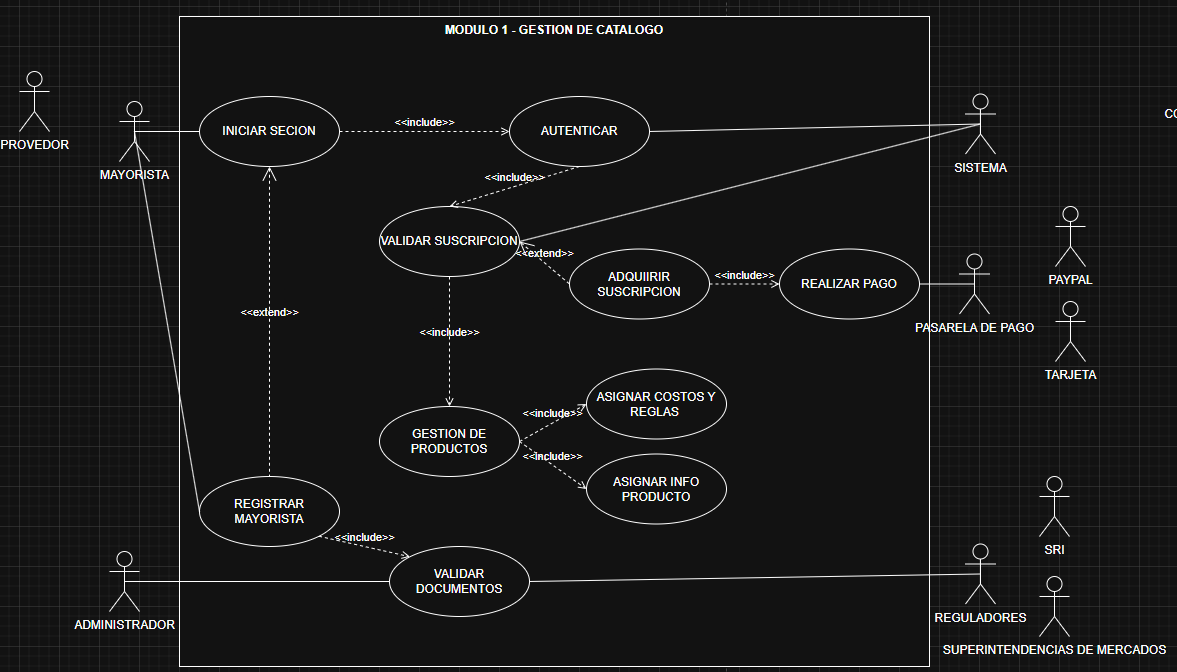
\includegraphics[width=0.45\textwidth]{CASO DE USO 1.png}
\hspace{0.05\textwidth}
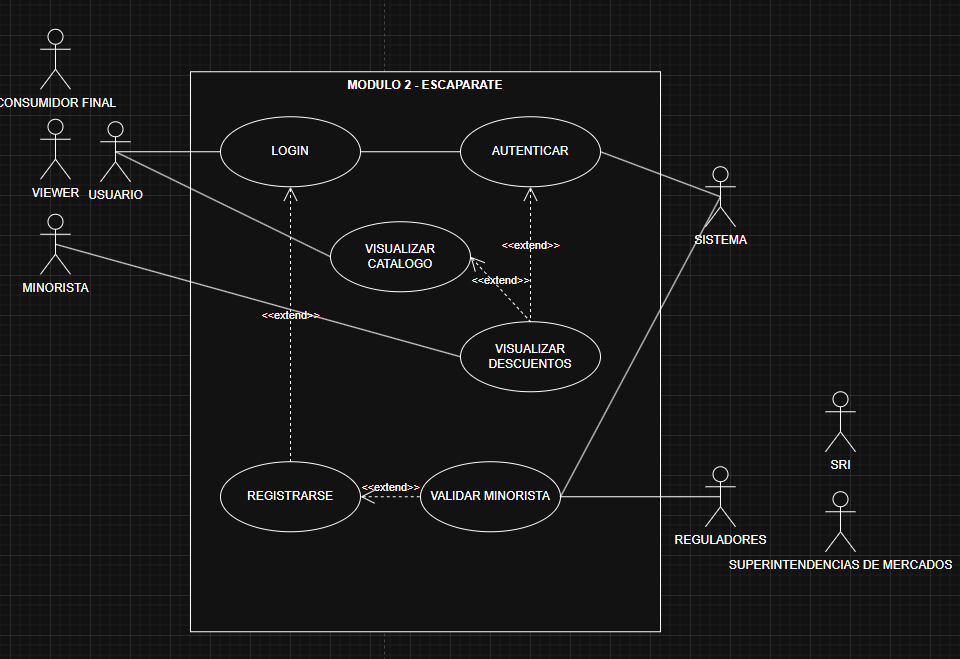
\includegraphics[width=0.45\textwidth]{CASO DE USO 2.png}
\caption{Casos de Uso 1 y 2 del Sistema Bazar B2B}
\end{figure}

\begin{figure}[htbp]
\centering
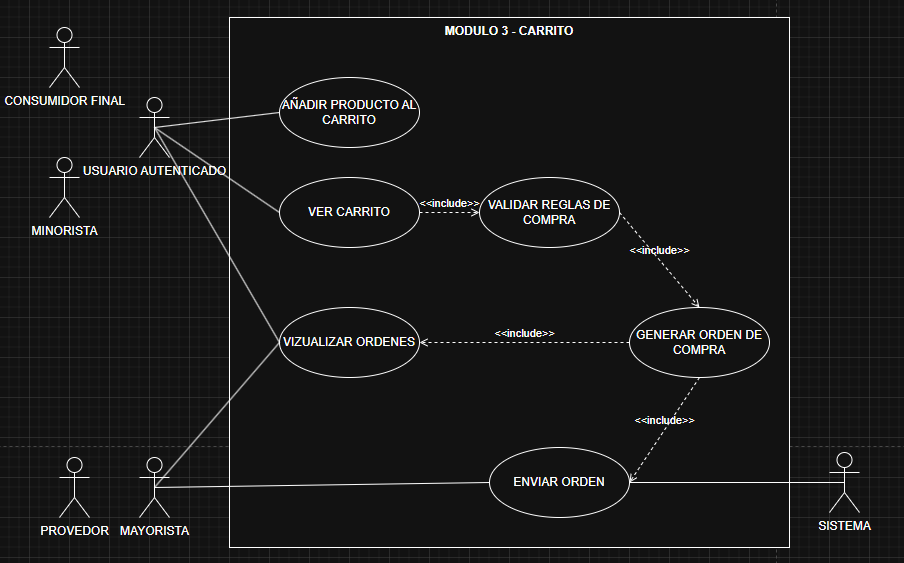
\includegraphics[width=0.45\textwidth]{CASO DE USO 3.png}
\hspace{0.05\textwidth}
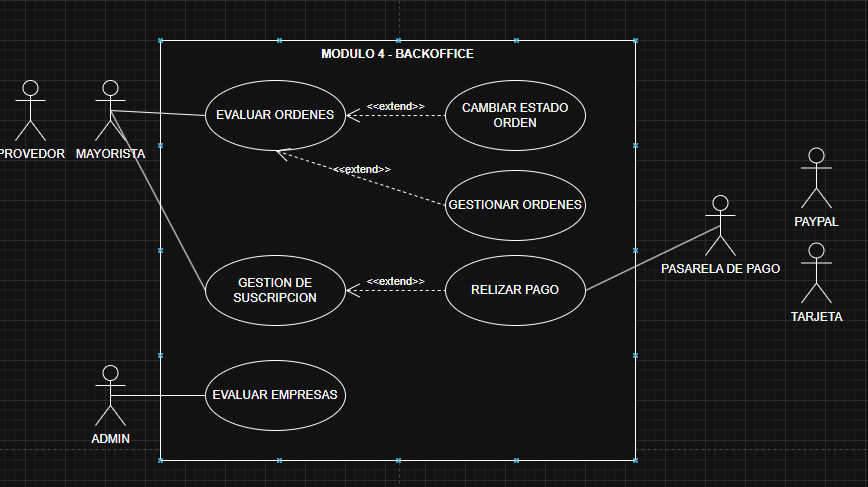
\includegraphics[width=0.45\textwidth]{CASO DE USO 4.png}
\caption{Casos de Uso 3 y 4 del Sistema Bazar B2B}
\end{figure}

\section{Sprint}
El primer Sprint se enfoca en el desarrollo del Catálogo Público con precios por Rol y el Motor de Carrito Inteligente (con MOQ validado), usando datos simulados (\textit{Mock Data}) en una primera etapa para cumplir con los plazos de entrega a los auspiciantes.

\section{Diagramas: Clases y BD (diseño lógico) - Preguntas y respuesta al diagrama}

\subsection*{Diagrama de Clases}

\begin{verbatim}
classDiagram
    %% Relaciones
    Usuario "1" -- "0..1" Suscripcion : tiene
    PlanSuscripcion "1" -- "0..*" Suscripcion : genera
    Usuario "1" -- "0..*" Producto : publica (Mayorista)
    Usuario "1" -- "0..*" OrdenCompra : realiza (Cliente)
    OrdenCompra "1" -- "1..*" DetalleOrden : contiene
    Producto "1" -- "0..*" DetalleOrden : pertenece a
    Producto "1" -- "0..*" ItemCarrito : en
    Carrito "1" -- "0..*" ItemCarrito : agrupa
    Usuario "1" -- "1" Carrito : posee

    class Usuario {
        +UUID id
        +String nombre_empresa
        +String email
        +String password
        +Enum rol (Admin, Mayorista, Minorista, Consumidor)
        +String ruc_nit
        +Enum estado_verificacion (Pendiente, Aprobado)
        +iniciar_sesion()
        +solicitar_verificacion()
    }

    class PlanSuscripcion {
        +UUID id
        +String nombre_plan
        +Decimal precio_mensual
        +Int limite_productos
        +Boolean destacado
    }

    class Suscripcion {
        +UUID id
        +Date fecha_inicio
        +Date fecha_fin
        +Enum estado (Activa, Vencida)
        +procesar_pago()
        +verificar_vigencia()
    }

    class Producto {
        +UUID id
        +String sku
        +String titulo
        +Text descripcion
        +String imagen_url
        +Decimal precio_base
        +Decimal precio_minorista
        +Int moq_cantidad_minima
        +Int multiplo_lote
        +Int stock_disponible
        +calcular_precio_segun_rol(rol_usuario)
    }

    class Carrito {
        +UUID id
        +DateTime ultima_actualizacion
        +vaciar_carrito()
        +generar_orden_compra()
    }

    class ItemCarrito {
        +UUID id
        +Int cantidad_solicitada
        +Decimal subtotal
        +validar_regla_moq() Boolean
        +validar_multiplo_lote() Boolean
    }

    class OrdenCompra {
        +UUID id
        +String numero_orden
        +DateTime fecha_creacion
        +Enum estado_orden (Pendiente, Preparacion, Entregado)
        +Decimal total_calculado
        +String metodo_pago_acordado
        +cambiar_estado(nuevo_estado)
    }

    class DetalleOrden {
        +UUID id
        +Int cantidad
        +Decimal precio_unitario_congelado
        +Decimal subtotal
    }
\end{verbatim}

\subsection*{Pregunta 1: Restricciones de Suscripción en Alta Demanda B2B}
\textbf{Escenario:} Un usuario se registra como \textit{Mayorista}, pasa el proceso de validación y contrata un plan básico. Intenta ejecutar una carga masiva para publicar 400 productos en el catálogo, pero su plan tiene un límite estricto de 100 productos.\\
\textbf{Pregunta:} ¿Qué flujo exacto de clases, métodos y atributos interviene para autorizar su cuenta, procesar su membresía y posteriormente denegar la subida del producto número 101?\\
\textbf{Resolución:}
\begin{itemize}
    \item \textbf{Quiénes intervienen:} \texttt{Usuario}, \texttt{PlanSuscripcion}, \texttt{Suscripcion} y \texttt{Producto}.
    \item \textbf{Por qué y cómo:}
    \begin{enumerate}
        \item El \texttt{Usuario} (con atributo \texttt{rol = Mayorista} y \texttt{estado\_verificacion = Pendiente}) invoca el método \texttt{solicitar\_verificacion()}. Una vez aprobado (\texttt{estado\_verificacion = Aprobado}), se le permite adquirir un plan.
        \item Se crea una instancia de \texttt{Suscripcion} a partir de un \texttt{PlanSuscripcion} seleccionado. El pago se consolida llamando a \texttt{Suscripcion.procesar\_pago()}, lo que cambia su \texttt{estado} a \texttt{Activa}.
        \item Al momento de la carga masiva, por cada nuevo \texttt{Producto} que el Mayorista intenta instanciar (relación \textit{Usuario 1 -> 0..* Producto}), el sistema debe verificar la cantidad de productos actuales asociados a ese ID de Usuario.
        \item El sistema cruza este conteo con el atributo \texttt{limite\_productos} de la clase \texttt{PlanSuscripcion} vinculada a su \texttt{Suscripcion} activa. Al llegar al producto 101, la validación falla a nivel de negocio y se bloquea la creación de más instancias de \texttt{Producto}.
    \end{enumerate}
\end{itemize}

\subsection*{Pregunta 2: Colisión de Reglas de Venta B2B (MOQ y Lotes)}
\textbf{Escenario:} Un \texttt{Minorista} está navegando por el catálogo e intenta agregar a su carrito 85 unidades de un suministro médico. El Mayorista configuró el producto con un \texttt{moq\_cantidad\_minima} de 50 unidades y un \texttt{multiplo\_lote} de 20 unidades.\\
\textbf{Pregunta:} ¿Cómo reacciona el modelo de clases al intentar añadir estas 85 unidades y qué mecanismos garantizan que no se pueda evadir la regla antes de generar la orden de compra?\\
\textbf{Resolución:}
\begin{itemize}
    \item \textbf{Quiénes intervienen:} \texttt{Producto}, \texttt{Carrito} y \texttt{ItemCarrito}.
    \item \textbf{Por qué y cómo:}
    \begin{enumerate}
        \item El \texttt{Carrito} del Minorista intenta crear una nueva instancia de \texttt{ItemCarrito} con el atributo \texttt{cantidad\_solicitada = 85}.
        \item Inmediatamente, el \texttt{ItemCarrito} debe invocar sus métodos de validación contra el \texttt{Producto} asociado:
        \begin{itemize}
            \item Ejecuta \texttt{validar\_regla\_moq()}: Compara 85 contra el \texttt{moq\_cantidad\_minima} (50). Esta prueba es \textbf{exitosa} (85 >= 50).
            \item Ejecuta \texttt{validar\_multiplo\_lote()}: Verifica si 85 es divisible exactamente por el \texttt{multiplo\_lote} (20). Esta prueba \textbf{falla} (85 \% 20 != 0).
        \end{itemize}
        \item Debido a que falla la regla de lote, la instancia del \texttt{ItemCarrito} es rechazada o entra en error, evitando que se sume al \texttt{subtotal}. En consecuencia, el método \texttt{generar\_orden\_compra()} de la clase \texttt{Carrito} no podrá procesar ítems inválidos.
    \end{enumerate}
\end{itemize}

\subsection*{Pregunta 3: Congelamiento de Precios e Inflación}
\textbf{Escenario:} Un \texttt{Minorista} y un \texttt{Consumidor} añaden el mismo \texttt{Producto} a sus respectivos carritos el día lunes. El martes, el \texttt{Mayorista} actualiza el precio del producto subiéndolo un 15\%. El miércoles, ambos clientes deciden pagar y concretar la orden basándose en lo que vieron el lunes.\\
\textbf{Pregunta:} ¿De qué manera el diagrama resuelve la visualización de precios dinámicos por rol y cómo evita que el aumento de precio del martes afecte las órdenes procesadas el miércoles (o garantiza el precio histórico)?\\
\textbf{Resolución:}
\begin{itemize}
    \item \textbf{Quiénes intervienen:} \texttt{Producto}, \texttt{Usuario}, \texttt{ItemCarrito} y \texttt{DetalleOrden}.
    \item \textbf{Por qué y cómo:}
    \begin{enumerate}
        \item \textbf{Cálculo dinámico:} El lunes, al visualizar el catálogo, se invoca el método \texttt{Producto.calcular\_precio\_segun\_rol(rol\_usuario)}. El sistema lee el atributo \texttt{rol} de cada \texttt{Usuario}. Al Minorista le retorna el \texttt{precio\_minorista} y al Consumidor el \texttt{precio\_base}.
        \item \textbf{Transacción (El congelamiento):} El miércoles, cuando invocan \texttt{Carrito.generar\_orden\_compra()}, la aplicación debe recalcular el total al momento del \textit{checkout}. Si la política del negocio es no respetar el precio del carrito antiguo, se vuelve a invocar \texttt{calcular\_precio\_segun\_rol()}, tomando el nuevo precio con el 15\% de aumento.
        \item \textbf{Persistencia:} Una vez efectuado el pago, los datos del \texttt{ItemCarrito} se transforman en una instancia de \texttt{DetalleOrden}. Aquí interviene un atributo vital: \texttt{precio\_unitario\_congelado}. Este atributo guarda el valor exacto pagado, independientemente de si el \texttt{Producto} cambia su precio futuro, garantizando la inmutabilidad de la \texttt{OrdenCompra} y protegiendo la auditoría financiera.
    \end{enumerate}
\end{itemize}

\subsection*{Pregunta 4: Ciclo de Vida de la Orden y Cancelaciones Tardías}
\textbf{Escenario:} Un cliente paga por una orden (quedando en estado Pendiente). Horas después, el \texttt{Mayorista} inicia la preparación del envío. En ese mismo instante, el cliente intenta cancelar la compra desde su interfaz.\\
\textbf{Pregunta:} Basado en la clase \texttt{OrdenCompra}, ¿cómo se gestiona la máquina de estados de este documento y por qué la estructura de datos impide inconsistencias entre ambos actores?\\
\textbf{Resolución:}
\begin{itemize}
    \item \textbf{Quiénes intervienen:} \texttt{OrdenCompra}, \texttt{Usuario} (Cliente) y \texttt{Usuario} (Mayorista/Admin).
    \item \textbf{Por qué y cómo:}
    \begin{enumerate}
        \item La orden se instanció con un identificador único (\texttt{UUID id}) y el atributo \texttt{estado\_orden} se inicializó en \texttt{Pendiente}.
        \item El Mayorista interviene ejecutando el método \texttt{cambiar\_estado(nuevo\_estado)}, actualizando el enum a \texttt{Preparacion}.
        \item Cuando el cliente intenta cancelar, el sistema debe consultar el estado actual de la \texttt{OrdenCompra}. Como el atributo ya mutó a \texttt{Preparacion}, la lógica de negocio detrás de \texttt{cambiar\_estado()} evaluará que no se puede transicionar de \texttt{Preparacion} a un estado de cancelación (flujo no permitido directamente).
        \item El modelo lo resuelve de forma centralizada: al tener un solo estado (\texttt{estado\_orden}) alojado en la cabecera del documento (\texttt{OrdenCompra}), asegura que no haya colisiones de estados paralelos entre el \texttt{Carrito} del cliente y el Backoffice del mayorista.
    \end{enumerate}
\end{itemize}

\subsection*{Pregunta 5: Carritos Abandonados y Retención de Stock}
\textbf{Escenario:} Un cliente \texttt{Minorista} añade todo el stock disponible (1000 unidades) de un producto muy solicitado a su carrito, pero cierra el navegador sin comprar, dejando su sesión ``en el limbo''. Otros compradores ven el producto como ``Agotado''.\\
\textbf{Pregunta:} ¿Qué atributos presentes en el modelo de datos permiten a los procesos de Backoffice solucionar este cuello de botella y liberar el inventario retenido?\\
\textbf{Resolución:}
\begin{itemize}
    \item \textbf{Quiénes intervienen:} \texttt{Carrito}, \texttt{ItemCarrito} y \texttt{Producto}.
    \item \textbf{Por qué y cómo:}
    \begin{enumerate}
        \item El principal aliado para este escenario es el atributo \texttt{ultima\_actualizacion} (tipo DateTime) ubicado en la clase \texttt{Carrito}.
        \item El sistema puede ejecutar una tarea programada (Cron Job) que escanee todas las instancias de \texttt{Carrito} buscando aquellas cuya \texttt{ultima\_actualizacion} exceda un tiempo prudencial (ej. 24 horas sin actividad).
        \item Al detectar el carrito abandonado, el sistema interviene ejecutando el método \texttt{vaciar\_carrito()}.
        \item Este método tiene un efecto en cascada: destruye las instancias de \texttt{ItemCarrito} vinculadas mediante la relación de agregación y toma la \texttt{cantidad\_solicitada} que estaba retenida para sumarla nuevamente al atributo \texttt{stock\_disponible} de la clase \texttt{Producto}, habilitando las ventas para otros clientes.
    \end{enumerate}
\end{itemize}

\section{Diagrama de componentes}

\subsection*{Arquitectura de Componentes}

\begin{verbatim}
graph TD
    subgraph Frontend [Capa Frontend - Next.js]
        UI[Interfaz UI y Componentes]
        AuthFront[Gestor de Roles y Estado]
        Escaparate[Módulo Escaparate Público]
        Carrito[Módulo Carrito y MOQ]
        Backoffice[Dashboard Administrador]
    end

    subgraph Backend [Capa Backend - Django REST]
        API[API Gateway / Enrutador URLs]
        Security[Servicio Autenticación JWT]
        ProductSVC[Controlador de Catálogo y Reglas]
        OrderSVC[Controlador de Transacciones]
        ORM[Django ORM - Capa de Datos]
    end

    subgraph Database [Capa Persistencia]
        DB[(PostgreSQL)]
    end

    UI --> AuthFront
    UI --> Escaparate
    UI --> Carrito
    UI --> Backoffice

    API --> Security
    API --> ProductSVC
    API --> OrderSVC

    Security --> ORM
    ProductSVC --> ORM
    OrderSVC --> ORM

    Escaparate -.->|Consulta productos| API
    Carrito -.->|Envía órdenes| API
    Backoffice -.->|Gestión B2B| API
    AuthFront -.->|Valida Token| API

    ORM -->|Lectura / Escritura| DB
\end{verbatim}

\begin{figure}[htbp]
\centering
\includegraphics[width=\textwidth]{Diagrama de componentes.png}
\caption{Diagrama de Componentes del Sistema Bazar B2B}
\end{figure}

\section{Arquitectura lógica y física (propuesta)}
\textbf{Arquitectura lógica:} Patrón MVC o Arquitectura Limpia, desacoplando la lógica de negocio del Backend en Python/Django, de la vista gestionada en Next.js/React.\\
\textbf{Arquitectura física:} Despliegue en la nube. Frontend alojado en servicios como Vercel y Backend/BD en Supabase o servidores cloud de rápida provisión (Render/AWS).

\section{Prototipo de pantallas no funcional}

\begin{figure}[htbp]
\centering
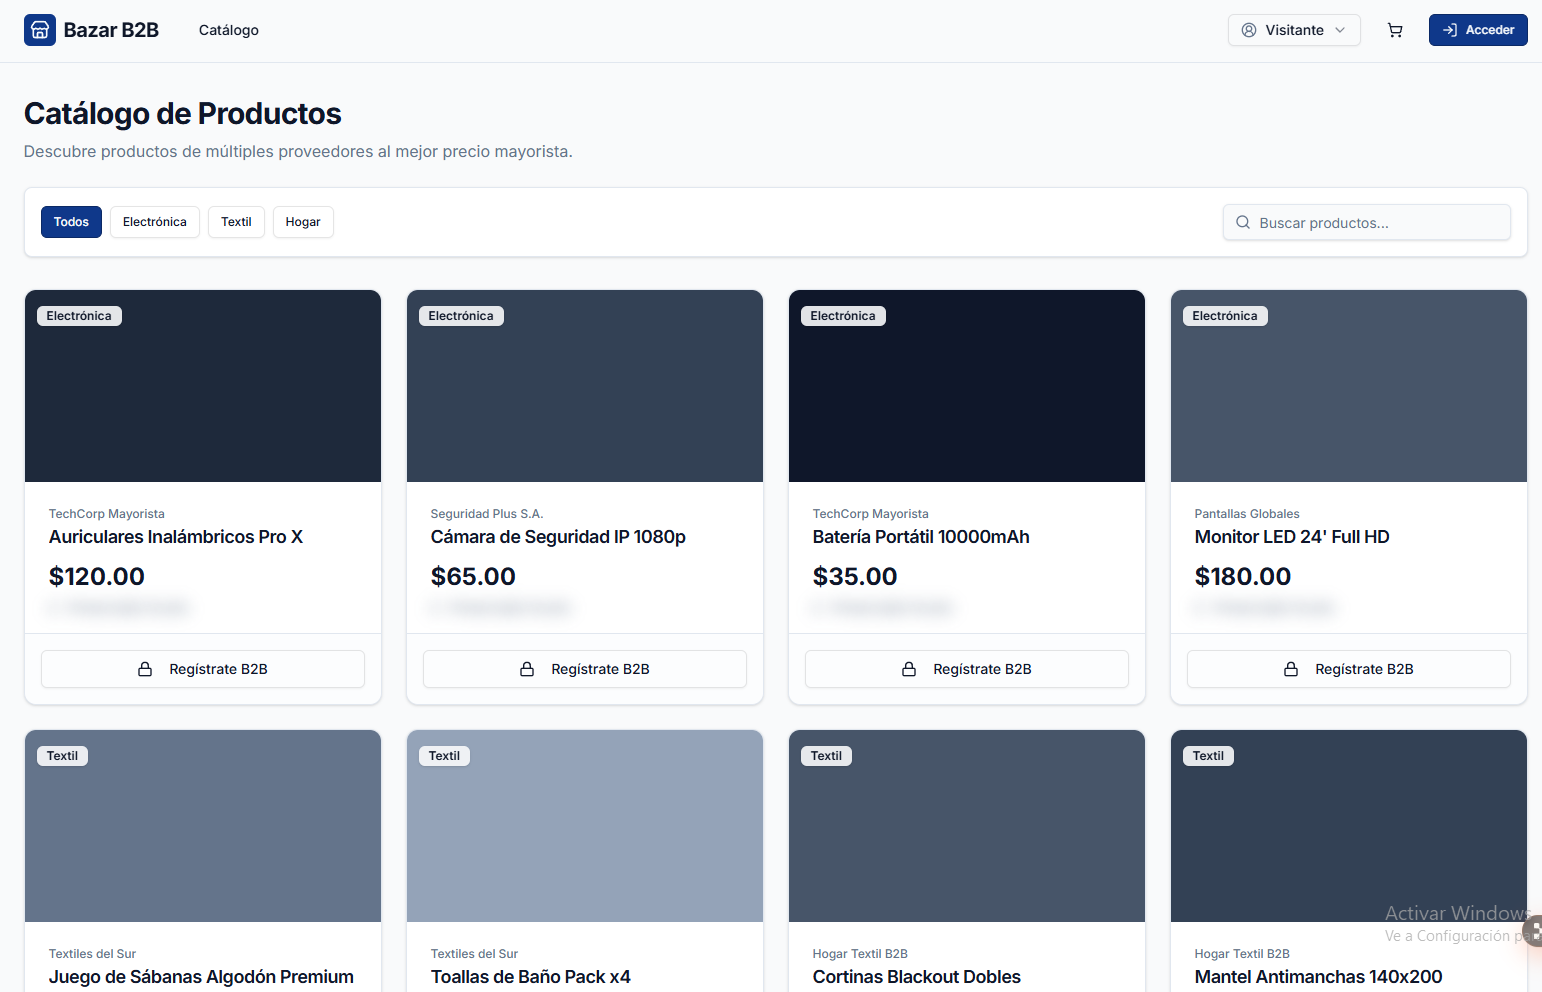
\includegraphics[width=0.9\textwidth]{PROTOTIPO1.png}
\caption{Prototipo 1: Vista de Catálogo Público}
\end{figure}

\begin{figure}[htbp]
\centering
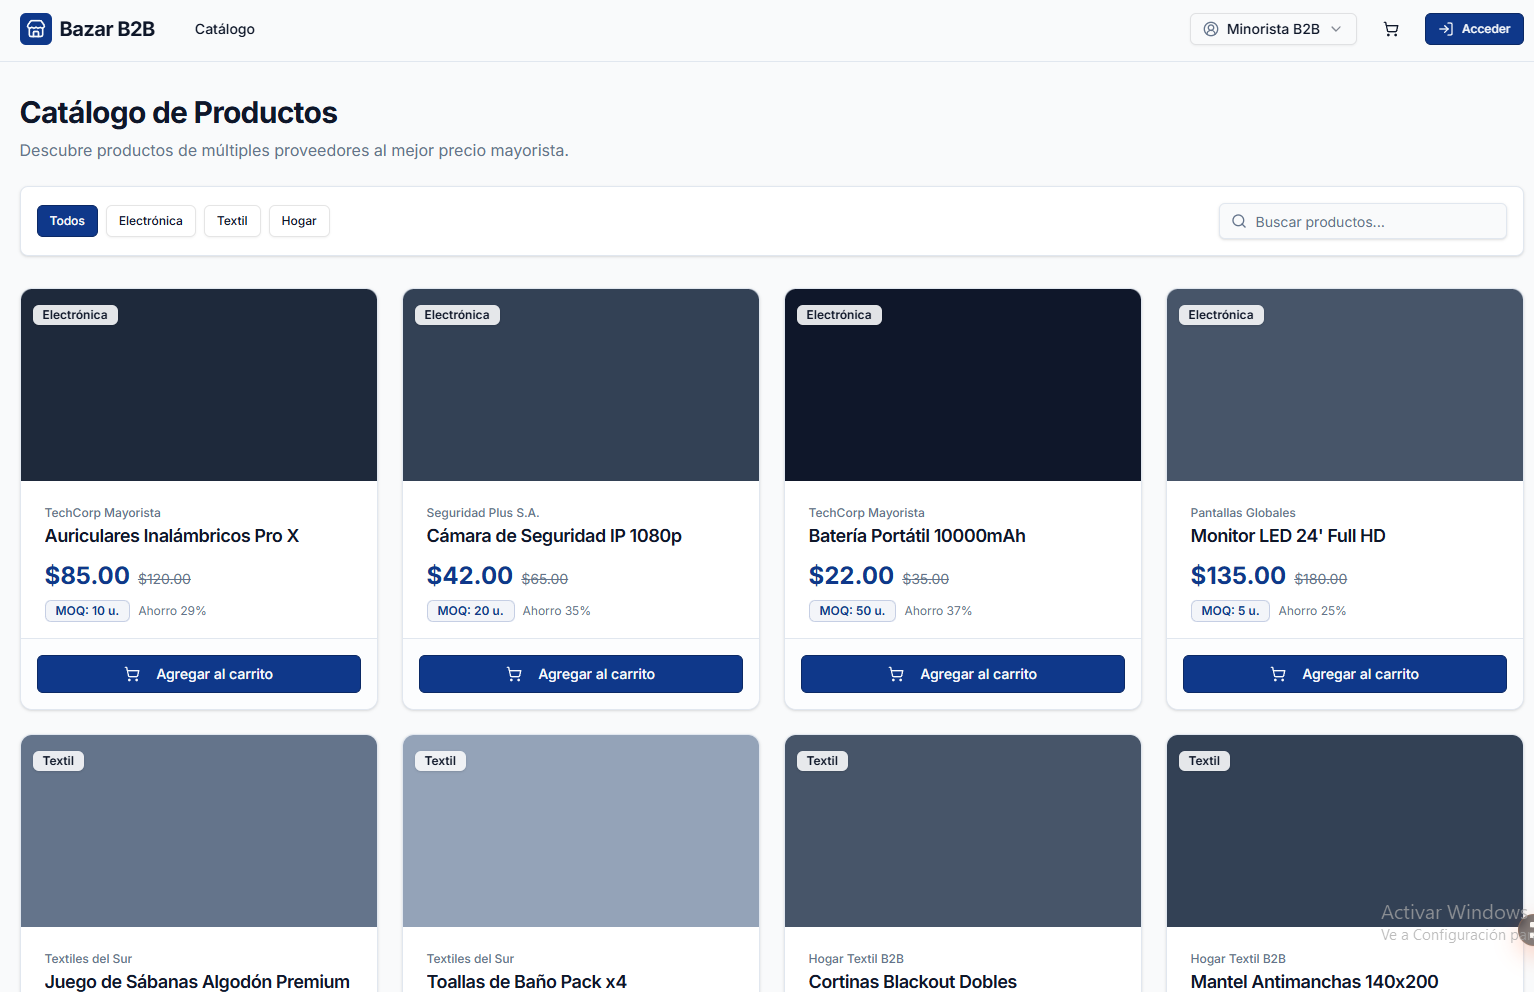
\includegraphics[width=0.9\textwidth]{PROTOTIPO2.png}
\caption{Prototipo 2: Carrito Inteligente MOQ y Checkout}
\end{figure}

\begin{figure}[htbp]
\centering
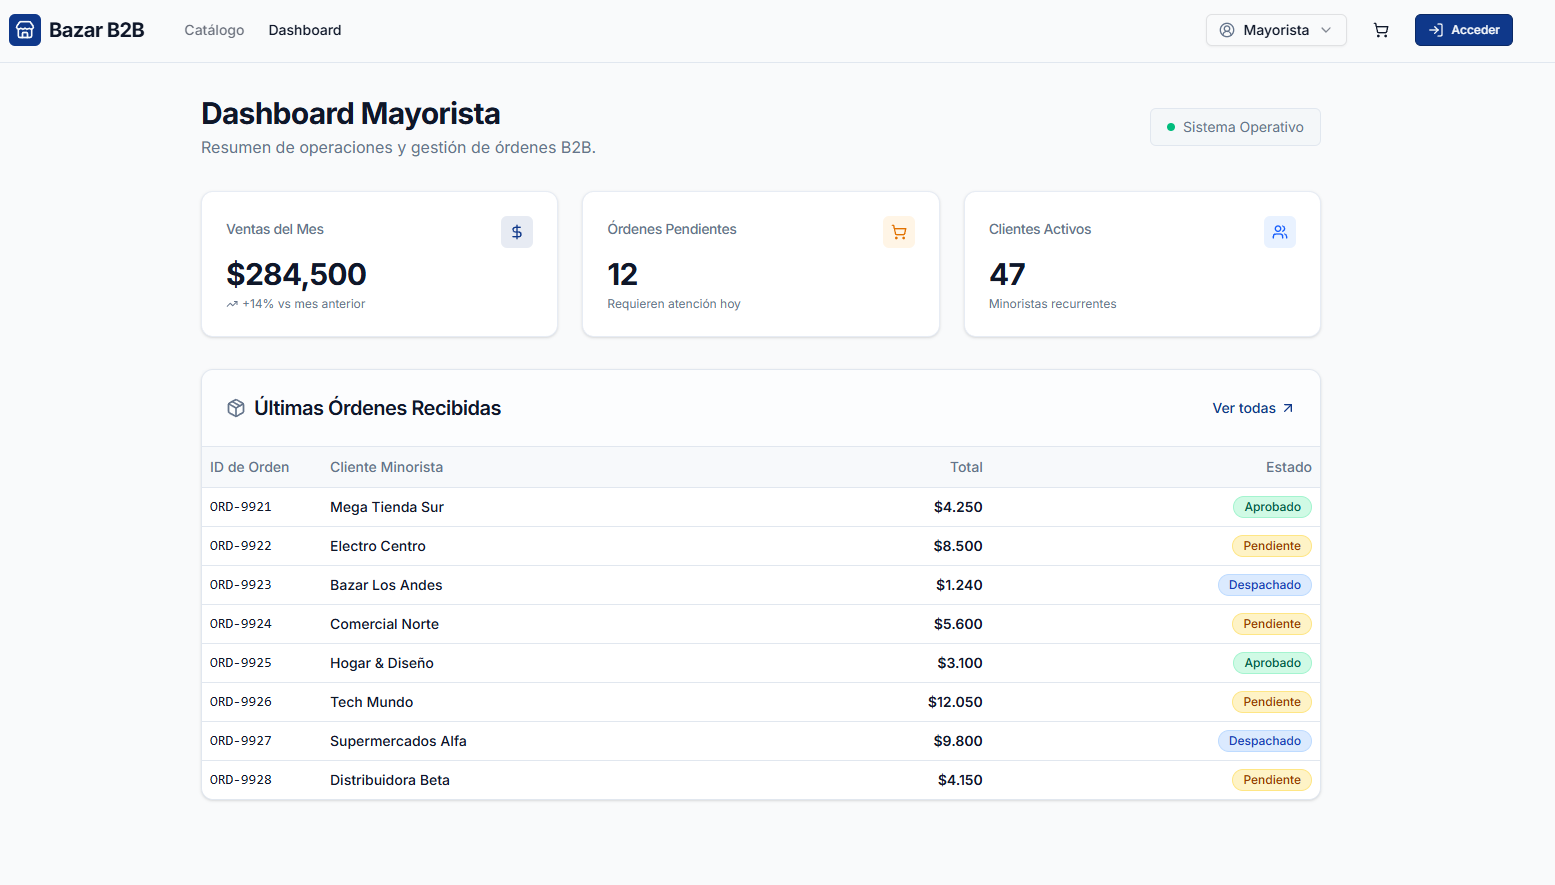
\includegraphics[width=0.9\textwidth]{PROTOTIPO3.png}
\caption{Prototipo 3: Dashboard Mayorista y Panel de Gestión}
\end{figure}

\end{document}
